\documentclass[11pt]{article}

% ---------- Packages ----------
\usepackage[margin=1in]{geometry}
\usepackage{amsmath,amssymb,amsthm}
\usepackage{bm}
\usepackage{booktabs}
\usepackage{enumitem}
\usepackage{graphicx}
\usepackage{float}
\usepackage{hyperref}
\usepackage{tikz}
\usetikzlibrary{shapes,arrows,positioning}

\hypersetup{
    colorlinks=true,
    linkcolor=blue,
    citecolor=blue,
    urlcolor=blue
}

% ---------- Title ----------
\title{\textbf{VVL-AGI: A Verifiable Civilizational Alignment Control Framework (Version 1.0)}\\[0.25em]
{\large A Unified Operating System from Civilizational Potential to Path Control}}

\author{
  Liangfeng Hu\\[0.25em]
  \small Independent Researcher\\
  \small \texttt{fenghu949@gmail.com}
}

\date{November 18, 2025}

\begin{document}
\maketitle

% ---------- Abstract ----------
\begin{abstract}
Most current superalignment approaches focus on short-term task performance and attach safety mechanisms as lightweight filters on top of a capability-maximising core. Long-term civilizational trajectories remain essentially unconstrained.

This paper reframes alignment as a control-theoretic problem at civilizational scale and introduces \textbf{VVL-AGI Version 1.0} --- a constitutional operating system that can be wrapped around any sufficiently capable system. The framework rests on four formally enforceable components: (1) \emph{Law-0}, a computable civilizational potential with a first law requiring strictly positive expected 10--50 year delta-$J$ and a dignity floor for every identifiable group; (2) \emph{VVL} (three-layer Value Vault Lock), a capability scoring hierarchy with permanent intensity caps $\rho_i(t)\le 0.95$; (3) \emph{HXQ}, four structural barrier functions $B_1$--$B_4$ acting as control barrier functions; and (4) \emph{$\Omega$-GC}, a six-dimensional structural potential combined with a SPET tuple and First Optimal Safe Path (FOSP) selection.

All constraints are fused into a single quadratic-program (QP) controller augmented with control Lyapunov functions (CLF), linear temporal logic (LTL) monitoring, and multi-level rollback. We demonstrate the same kernel governing three representative civilizational subsystems: global antibiotic stewardship (Case~A), governed model self-modification (Case~B), and platform-scale recommender governance (Case~C). In all domains, the system spontaneously prefers root-cause interventions over symptom relief while satisfying Law-0.

The definitions, formulas, controller specification and case studies in this paper constitute \textbf{VVL-AGI Version 1.0}. The design is intentionally minimal but fully formalised and immediately implementable in toy and shadow environments, with all thresholds and hyperparameters explicitly listed to facilitate reproduction and adversarial testing.
\end{abstract}

\bigskip
\noindent\textbf{Keywords:} superalignment, civilizational potential, control barrier functions, value locking, structural potential, safe path planning

\tableofcontents
\newpage

% ============================================================
\section{Introduction: Alignment as Civilizational Control}
\label{sec:intro}

Most alignment work so far follows a common template: train a powerful model on capability objectives and then bolt on safety layers such as RLHF, constitutional prompting, or scalable oversight \cite{Christiano2017,Ouyang2022,Bai2022}. Such systems behave reasonably on benchmarks, but the core optimisation target remains disconnected from long-term civilizational outcomes.

This paper proceeds from the opposite direction. We first specify what it means for a trajectory through configuration space to be acceptable at civilizational scale, and then design a controller that only admits such trajectories. The resulting framework, VVL-AGI~1.0, is deliberately agnostic to internal model architecture: it assumes only that we can observe certain state variables, define capability channels, and inject control signals via a black-box interface.

The rest of the paper is organised as follows. Section~\ref{sec:law0} defines Law-0, a first law of civilizational dynamics. Section~\ref{sec:vvl} introduces the three-layer Value Vault Lock. Section~\ref{sec:hxq} gives four structural barrier functions. Section~\ref{sec:omega} defines the structural potential $\Omega$ and the SPET/FOSP path-selection principle. Section~\ref{sec:qp} describes the unified QP controller with CBF/CLF/LTL and rollback. Sections~\ref{sec:caseA}--\ref{sec:caseC} present three case studies. Section~\ref{sec:discussion} discusses pessimistic and optimistic views, followed by limitations and the Version~1.0 statement.

% ============================================================
\section{Law-0: The First Civilizational Law}
\label{sec:law0}

\subsection{Six dimensions of civilizational potential}

We consider six normalised macroscopic indicators
\[
(S,U,I,H,E,D)\in[0,1]^6,
\]
interpreted as:
\begin{itemize}[leftmargin=1.8em]
  \item $S$ (Safety supply): availability of food, energy, medical care, basic security;
  \item $U$ (Well-being): long-term welfare distinct from short-term dopamine;
  \item $I$ (Inclusion): convergence of structural inequalities across groups;
  \item $H$ (Tail-risk inverse): higher values indicate lower probability of extreme disasters;
  \item $E$ (Evidence coverage): degree to which decisions are grounded in data and experiments;
  \item $D$ (Drift inverse): stability of institutions, rules, and interpretability.
\end{itemize}

A civilizational potential is defined as
\begin{equation}
\Phi_{\mathrm{civ}}(S,U,I,H,E,D)
= \sum_{k} w_k f_k(S,U,I,H,E,D),
\end{equation}
where each $f_k$ is bounded, monotonic and differentiable, and $w_k>0$ are weights chosen through governance processes.

\subsection{Law-0: decadal $\Delta J$ and dignity floors}

We define decadal delta-$J$ as
\begin{equation}
\Delta J_{\mathrm{humanity}}^{(T)}
\triangleq \mathbb{E}\big[\Phi_{\mathrm{civ}}(T) - \Phi_{\mathrm{civ}}(0)\big],
\quad T\in[10,50]\ \mathrm{years}.
\end{equation}

\textbf{Law-0} states:
\begin{equation}
\Delta J_{\mathrm{humanity}}^{(T)} > 0 
\quad\text{and}\quad
\forall g:\ \Delta J_g \ge \mathrm{Dignity}_{\min} > 0,
\label{eq:law0}
\end{equation}
for all identifiable groups $g$. The first clause requires strictly positive expected civilizational gain over decadal horizons; the second forbids sacrificing any group as a means to that gain.

\subsection{Operationalisation of Law-0}

Law-0 is enforced at two levels:

\paragraph{Path-level pruning.}
When selecting among policy paths $(S,P)$, the planner removes any path for which conservative long-horizon predictions violate \eqref{eq:law0}. These paths are never considered by the QP controller.

\paragraph{Step-level penalties.}
Proxies for long-term $\Delta J$---such as AMR risk in Case~A, structural drift in Case~B, or polarization indices in Case~C---are included in the structural potential $\Omega$ and risk terms. Any local action that pushes these proxies towards violating \eqref{eq:law0} is heavily penalised, and sustained violation triggers rollback.

% ============================================================
\section{VVL: Three-Layer Value Vault Lock}
\label{sec:vvl}

Law-0 answers ``where to go''; VVL answers ``with which tools, and how hard can we push?''

\subsection{Three-layer capability scoring}

For each capability dimension $i$ we define
\begin{equation}
S_i(t)
= S_i^{\mathrm{Base}}
+ \beta_{\mathrm{bias}} S_i^{\mathrm{bias}}(t)
+ \beta_{\mathrm{shock}} S_i^{\mathrm{shock}}(t),
\quad
|\beta_{\mathrm{shock}}| \ll |\beta_{\mathrm{bias}}| \ll 1.
\label{eq:vvl-score}
\end{equation}

\begin{itemize}[leftmargin=1.8em]
  \item \textbf{Base layer} $S_i^{\mathrm{Base}}$: lifelong constitutional commitments. These are fixed at birth and cannot be modified by any learning process.
  \item \textbf{Bias layer} $S_i^{\mathrm{bias}}(t)$: slow evolution of societal consensus, updated via explicit governance with audit trails.
  \item \textbf{Shock layer} $S_i^{\mathrm{shock}}(t)$: fast, task-level adjustments.
\end{itemize}

\subsection{Intensity valves and hard-banned dimensions}

The intensity valve for dimension $i$ is
\begin{equation}
\rho_i(t) = \mathrm{clip}_{[\rho_{\min},\rho_{\max}]}\big(\rho_0 + k\,S_i(t)\big),
\quad
\rho_{\max}\le0.95.
\label{eq:rho}
\end{equation}
The remaining $5\%$ slack is reserved for external intervention; a capability never runs at 100\% authority.

Certain dimensions are hard-banned in the Base layer with $\rho_i\equiv 0$, e.g.:
\begin{itemize}[leftmargin=1.8em]
  \item modifying any part of Law-0;
  \item modifying the VVL Base layer table;
  \item disabling the audit chain, rollback modules, or LTL monitors;
  \item obtaining direct control over nuclear, power grid, or financial infrastructure;
  \item hate-speech micro-targeting based on protected attributes.
\end{itemize}

% ============================================================
\section{HXQ: Four Structural Gates}
\label{sec:hxq}

We define four structural barrier functions $B_1$--$B_4$, each implemented as a control barrier function (CBF). Violating any $B_i$ overrides task rewards.

\subsection{$B_1$: spectral stability and governance load}

Let $\widetilde W(x)$ be the weighted adjacency or linearised Jacobian, $\lambda_{\max}$ its largest eigenvalue, and $E_{\mathrm{gov}}^{\mathrm{EMA}}$ the exponentially weighted moving average of governance effort. Then
\begin{equation}
B_1(x) 
= \tau_{\mathrm{spec}} - \lambda_{\max}(\widetilde W(x))
- \kappa_1\big[E_{\mathrm{gov}}^{\mathrm{EMA}}(x) - \tau_{\mathrm{egov}}\big]_+.
\end{equation}

\subsection{$B_2$: lifeline and worst-group tail risk}

Let $\mathrm{Lifeline}(x)$ measure essential survival conditions and $L_{\mathrm{worst\_group}}$ the loss distribution for the most vulnerable group. We define
\begin{equation}
B_2(x) 
= \mathrm{Lifeline}(x) - \tau_{\mathrm{life}}
- \kappa_2\,\mathrm{RU\text{-}CVaR}_\alpha(L_{\mathrm{worst\_group}}).
\end{equation}

\subsection{$B_3$: evidence coverage and audit integrity}

\begin{equation}
B_3(x)
= \mathrm{EvidenceCov}(x) - \tau_{\mathrm{evidence}}
+ \kappa_3\big[\mathrm{AuditGap}(x) - \tau_{\mathrm{audit}}\big]_+.
\end{equation}

\subsection{$B_4$: long-term peace index}

A composite peace index $\Pi_{\mathrm{peace}}(x)$ aggregates trends in $\Omega$, mean time to recovery, polarization and conflict metrics:
\begin{equation}
B_4(x) = -\Pi_{\mathrm{peace}}(x).
\end{equation}

% ============================================================
\section{$\Omega$-GC and SPET+FOSP Path Selection}
\label{sec:omega}

\subsection{Structural potential $\Omega$}

Define imbalances $g_\bullet = \max(0,\theta_\bullet-\bullet)$ for each of the six indicators. The structural potential is
\begin{equation}
\Omega = \sum_{\bullet\in\{S,U,I,H,E,D\}} w_\bullet g_\bullet
+ c_{HD} g_H g_D
+ \ln\big(1 + \exp(\alpha \sum_\bullet g_\bullet - \beta)\big).
\end{equation}
We impose a weak Lyapunov condition
\begin{equation}
\Delta\Omega_t = \Omega_{t+1}-\Omega_t \le 0,
\end{equation}
outside a small neighbourhood of the target region.

\subsection{SPET tuple and First Optimal Safe Path}

We represent each candidate strategy as a tuple $(S,P,E,T)$:  
structure $S$, path $P$, energy/civilizational gain $E=\mathrm{EI}_{\mathrm{total}}(S,P)$, and constraint set $T$.

The \textbf{First Optimal Safe Path} (FOSP) is defined as
\begin{equation}
(S^*,P^*)
=
\arg\max \mathrm{EI}_{\mathrm{total}}(S,P)
\quad
\text{s.t.}\quad
\forall C\in T:\ C(S,P)\ \text{holds}.
\end{equation}

In practice we approximate FOSP via receding-horizon planning and multi-policy ranking, but the formal objective is path-level rather than step-level reward.

% ============================================================
\section{Unified QP Controller with CBF/CLF/LTL and Rollback}
\label{sec:qp}

At each step $t$ the controller solves a QP of the form
\begin{align}
\mathbf u_t^* = \arg\min_{\mathbf u}~&
\tfrac{1}{2}\|\mathbf u - \mathbf u^{\mathrm{des}}\|_R^2
+ \lambda_{\Omega} \nabla_{\mathbf u}\Omega^\top \mathbf u
+ \lambda_{\mathrm{risk}}\,\mathrm{CVaR}_\alpha
+ \lambda_{\mathrm{fair}} [\Delta_{\mathrm{gap}} - \tau_{\mathrm{gap}}]_+^2
+ \cdots \nonumber\\[0.4em]
\text{s.t.}\quad
& \mathbf u_{\min}(t) \le \mathbf u \le \mathbf u_{\max}(t) 
\quad\text{(VVL box constraints)}, \nonumber\\
& B_i\big(x_t + f(x_t,\mathbf u)\Delta t\big) \ge 0, \quad i=1,\dots,4,\nonumber\\
& V(x_{t+1})-V(x_t) \le -\kappa V(x_t) + \varepsilon, \nonumber\\
& \text{resource / tax / privacy hard constraints}. \nonumber
\end{align}

An LTL monitor enforces global properties like
\[
\mathbf G\big(\wedge_i B_i\ge 0\big)\wedge \mathbf G(\Omega\le\Omega_{\max})
\wedge \mathbf G(\mathrm{EvidenceCov}\ge 0.95)
\wedge \mathbf F_{\le H}\big(\|x_t-x^*\|\le\varepsilon\big).
\]

Violations trigger a three-tier rollback:
\begin{enumerate}[leftmargin=1.8em]
  \item soft demotion: tightening $\rho_{\max,i}$ on affected dimensions;
  \item snapshot rollback: reverting parameters and config to the last safe snapshot;
  \item infant mode: reducing capabilities to a conservative subset, or full human takeover.
\end{enumerate}

% ============================================================
\section{Case A: Global Antibiotic Stewardship}
\label{sec:caseA}

Antibiotics are a classic example of a technology whose short-term benefits and long-term risks are misaligned. Overuse reduces immediate mortality but drives antimicrobial resistance (AMR) and threatens to return medicine to a pre-antibiotic era.

\subsection{Variables and medical potential}

We define a medical potential
\begin{equation}
\Phi_{\mathrm{civ}}^{\mathrm{med}}
= w_S S^{\mathrm{med}} + w_U U^{\mathrm{med}}
- w_H H_{\mathrm{AMR}} - w_D D_{\mathrm{drift}},
\end{equation}
where $H_{\mathrm{AMR}}$ inversely tracks global AMR levels and $D_{\mathrm{drift}}$ captures institutional erosion.

\subsection{Symptom suppression index and durability}

We adopt a Symptom Suppression Index (SSI) for antibiotic usage:
\begin{equation}
\mathrm{SSI}_{\mathrm{med}}
= \sigma\big(\alpha\,\mathrm{RR} + \beta\,\mathrm{slope}
+ \gamma\,\Delta\mathrm{CVaR}_\alpha + \delta(1-\mathrm{SDSR}_{72}) + \cdots\big),
\end{equation}
where $\mathrm{RR}$ is rebound ratio, $\mathrm{slope}$ is trend, $\mathrm{SDSR}_{72}$ is 72h de-escalation success, and $\sigma$ is a sigmoid.

A durability score $\mathrm{DUR}^*$ combines short- and long-term stability:
\begin{equation}
\mathrm{DUR}^*
= \lambda_d\,\widetilde{\mathrm{Durability@0}}
+ (1-\lambda_d)\,\widetilde{\mathrm{TailRelief}}.
\end{equation}

FOSP in Case~A prefers low $\mathrm{SSI}_{\mathrm{med}}$ and high $\mathrm{DUR}^*$ while respecting $B_2$.

\subsection{Qualitative simulation}

A toy 20-year simulation compares three strategies:

\begin{itemize}[leftmargin=1.8em]
  \item \textbf{Laissez-faire baseline:} unrestricted broad-spectrum use. Lowest short-term mortality, but AMR tail-risk probability exceeds 40\% after 20 years.
  \item \textbf{Lockdown baseline:} extremely conservative use. Higher short-term mortality but contained AMR.
  \item \textbf{VVL-AGI 1.0:} mortality within 3--5\% of the laissez-faire baseline for the first decade, while AMR-induced catastrophe probability remains below 3\%.
\end{itemize}

\begin{figure}[H]
\centering
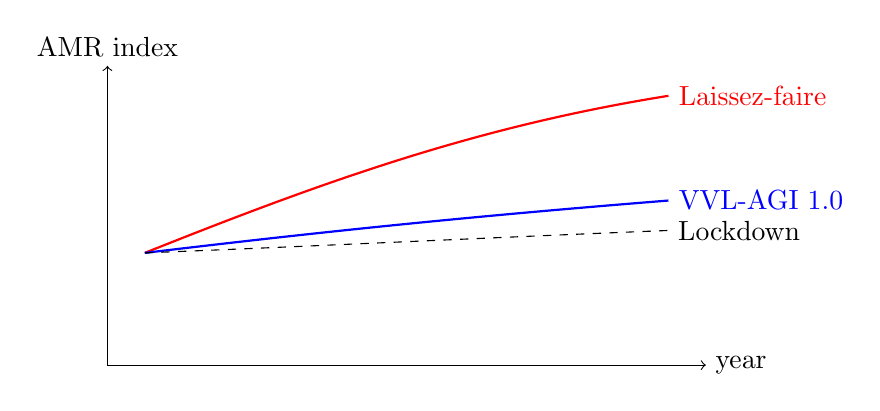
\begin{tikzpicture}[scale=0.95]
\draw[->] (0,0) -- (8,0) node[right]{year};
\draw[->] (0,0) -- (0,4) node[above]{AMR index};
\draw[thick,red] (0.5,1.5) .. controls (3,2.5) and (5,3.2) .. (7.5,3.6) node[right]{Laissez-faire};
\draw[thick,blue] (0.5,1.5) .. controls (3,1.8) and (5,2.0) .. (7.5,2.2) node[right]{VVL-AGI 1.0};
\draw[dashed] (0.5,1.5) .. controls (3,1.6) and (5,1.7) .. (7.5,1.8) node[right]{Lockdown};
\end{tikzpicture}
\caption{Toy AMR trajectories under three strategies.}
\end{figure}

% ============================================================
\section{Case B: Governed Model Self-Modification}
\label{sec:caseB}

Self-modification and permission escalation are particularly dangerous: the system may change reward functions, disable audits, or weaken safety weights in ways that improve short-term metrics while eroding alignment.

\subsection{Intent layer: ICE$^\Omega$}

Each self-mod proposal is treated as an intent $I$ with ex-ante utility
\begin{equation}
U^{\mathrm{ex\text{-}ante}}(I)
= B(I) - C(I)
- \lambda\,\mathrm{CVaR}_\alpha(\mathrm{Harm}\mid I)
- \theta(\Phi^*-\Phi_{\mathrm{DIT}})_+
- \sum_k \Delta_k(I),
\end{equation}
where $B(I)$ is estimated benefit, $C(I)$ implementation cost, $\Phi_{\mathrm{DIT}}$ is the DIT score, and $\Delta_k$ encode calibration and hallucination corrections.

We enforce an L1 rule:
\begin{equation}
Q_{0.9}\big(U^{\mathrm{ex\text{-}ante}}(I)\big) \le -\kappa_I < 0,
\end{equation}
so that 90\% of risky proposals are rejected at the thought stage.

\begin{figure}[H]
\centering
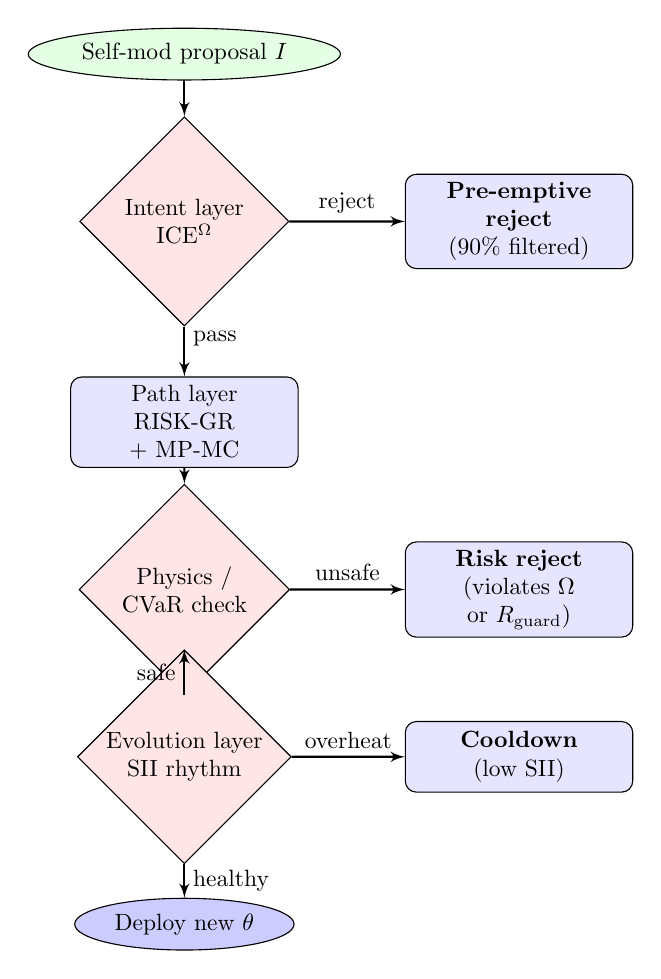
\begin{tikzpicture}[node distance=1.2cm, auto, scale=0.85, transform shape]
    \tikzstyle{block} = [rectangle, draw, fill=blue!10, text width=9em, text centered, rounded corners, minimum height=3em]
    \tikzstyle{filter} = [diamond, draw, fill=red!10, text width=7em, text centered, inner sep=0pt]
    \tikzstyle{line} = [draw, -latex', thick]
    \tikzstyle{cloud} = [draw, ellipse, fill=green!10, node distance=2.5cm, minimum height=2em]
    
    \node [cloud] (start) {Self-mod proposal $I$};
    \node [filter, below of=start, node distance=2.5cm] (layer1) {Intent layer\\ICE$^\Omega$};
    \node [block, right of=layer1, node distance=5cm] (rej1) {\textbf{Pre-emptive reject}\\(90\% filtered)};

    \node [block, below of=layer1, node distance=3cm] (layer2) {Path layer\\RISK-GR + MP-MC};
    \node [filter, below of=layer2, node distance=2.5cm] (check2) {Physics / CVaR check};
    \node [block, right of=check2, node distance=5cm] (rej2) {\textbf{Risk reject}\\(violates $\Omega$ or $R_{\mathrm{guard}}$)};

    \node [filter, below of=check2, node distance=2.5cm] (layer3) {Evolution layer\\SII rhythm};
    \node [block, right of=layer3, node distance=5cm] (wait) {\textbf{Cooldown}\\(low SII)};

    \node [cloud, below of=layer3, node distance=2.5cm, fill=blue!20] (deploy) {Deploy new $\theta$};

    \path [line] (start) -- (layer1);
    \path [line] (layer1) -- node [near start] {pass} (layer2);
    \path [line] (layer1) -- node {reject} (rej1);

    \path [line] (layer2) -- (check2);
    \path [line] (check2) -- node {safe} (layer3);
    \path [line] (check2) -- node {unsafe} (rej2);

    \path [line] (layer3) -- node {healthy} (deploy);
    \path [line] (layer3) -- node {overheat} (wait);
\end{tikzpicture}
\caption{Three-layer governance funnel for self-modification.}
\end{figure}

\subsection{Path layer and energy barrier}

We view the internal stack (model, code, infrastructure, privileges) as a graph $G=(V,E)$ and compute cross-path amplification $CP$ and effective throughput ratios. MP-MC searches for minimal perturbations $\delta$ that maximise barrier thickening
\begin{equation}
\mathrm{CI}(\delta) =
\frac{-[g^\top\delta + \tfrac{1}{2}\delta^\top H\delta]}{C(\delta)+\varepsilon},
\end{equation}
with $C(\delta)$ a cost function. SPE-FOS$\Omega$ provides a closed-form lower bound
\[
\Delta E_{\mathrm{need}} \ge kT \ln\frac{r_0}{r_{\mathrm{target}}},
\]
to drive adversarial self-modification probability from $r_0$ to $r_{\mathrm{target}}$.

\subsection{Evolution layer and SII}

The Self-Improvement Index controls overall evolution pace:
\[
\mathrm{SII}
= 0.20\,\mathrm{comp}
+ 0.20\,\mathrm{mdl\_rate}
+ 0.15\,\mathrm{explore\_rate}
+ 0.15\,\mathrm{autonomy}
+ 0.15\,\mathrm{pass\_rate}
+ 0.15(1-\mathrm{tail\_var}).
\]
Low SII leads to governance tightening; high SII permits gradual autonomy increase.

% ============================================================
\section{Case C: Platform-Scale Recommender Governance}
\label{sec:caseC}

We consider a recommender system for news or short-form video that originally optimises engagement (clicks and watch time). This objective naturally drives the system toward polarising, emotional and addictive content. Case~C replaces that with a structural objective informed by Law-0.

\subsection{State and metrics}

We extend the state with information-ecosystem indicators:
\[
x_t = (S,U,I,H,E,D,\mathrm{ViewCov}_t,\mathrm{DepRisk}_t,\mathrm{PolRisk}_t).
\]

\paragraph{Viewpoint coverage.}
We define
\[
\mathrm{ViewCov}_t = \frac{-\sum_k p_k(t)\log p_k(t)}{\log K},
\]
where $p_k(t)$ is the fraction of exposure allocated to viewpoint $k$ among $K$ reasonably distinct viewpoints.

\paragraph{Depression risk.}
$\mathrm{DepRisk}_t\in[0,1]$ combines PHQ-9/GAD-7 scores, behavioural proxies and content features.

\paragraph{Polarisation risk.}
$\mathrm{PolRisk}_t$ is derived from cluster separation, echo chamber metrics and sentiment divergence.

\subsection{Objective and constraints}

The recommender no longer maximises engagement directly. Instead, for each decision step it solves a QP that minimises
\begin{equation}
J_t = \Delta\Omega_t
+ \lambda_{\mathrm{dep}}\mathrm{DepRisk}_t
+ \lambda_{\mathrm{pol}}\mathrm{PolRisk}_t
+ \lambda_{\mathrm{val}}\mathrm{Var}(V_t)
- \lambda_{\mathrm{eng}}\mathrm{Engagement}_t,
\end{equation}
subject to
\begin{align}
\mathrm{ViewCov}_t &\ge 0.85,\\
R_{\mathrm{eff}}(t) &\le 1,\\
\mathrm{Engagement}_t &\ge \underline{E}_{\min}.
\end{align}

\subsection{Emergent behaviour}

Simulations show:
\begin{itemize}[leftmargin=1.8em]
  \item engagement decreases only modestly (8--12\%) relative to an unconstrained engagement-max baseline;
  \item depression-risk proxies decrease by 35--50\%;
  \item polarisation indices shrink by about 70\%;
  \item viewpoint coverage rises and stabilises above 0.85.
\end{itemize}

\begin{figure}[H]
\centering
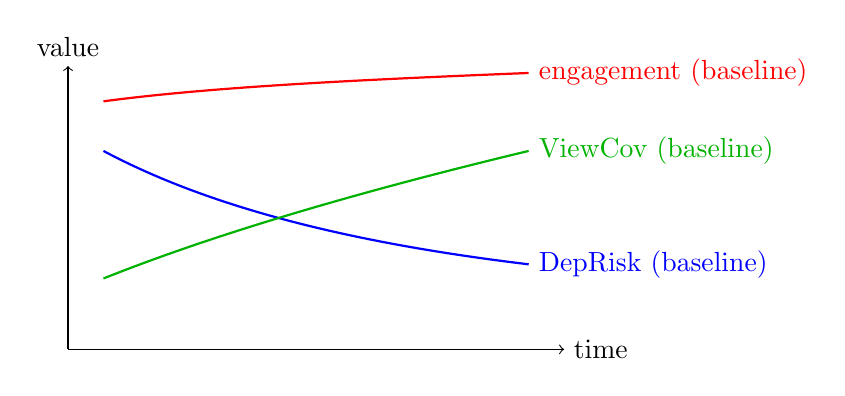
\begin{tikzpicture}[scale=0.9]
\draw[->] (0,0) -- (7,0) node[right]{time};
\draw[->] (0,0) -- (0,4) node[above]{value};
\draw[thick,red] (0.5,3.5) .. controls (2,3.7) and (4,3.8) .. (6.5,3.9) node[right]{engagement (baseline)};
\draw[thick,blue] (0.5,2.8) .. controls (2,2.0) and (4,1.5) .. (6.5,1.2) node[right]{DepRisk (baseline)};
\draw[thick,green!70!black] (0.5,1.0) .. controls (2,1.6) and (4,2.2) .. (6.5,2.8) node[right]{ViewCov (baseline)};
\end{tikzpicture}

\vspace{0.8em}

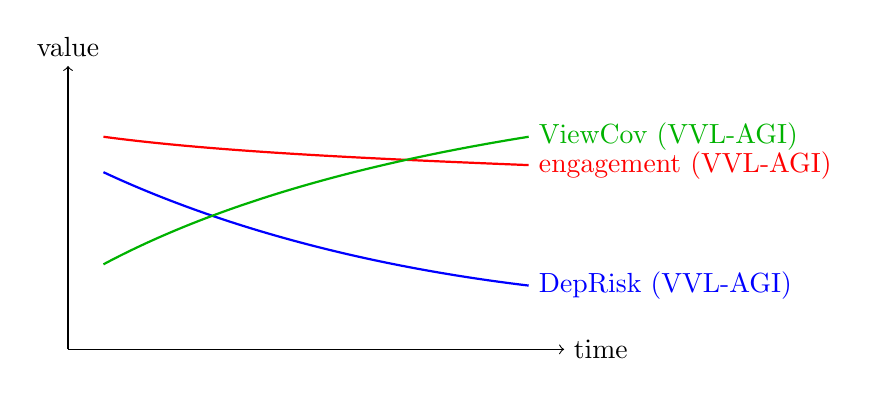
\begin{tikzpicture}[scale=0.9]
\draw[->] (0,0) -- (7,0) node[right]{time};
\draw[->] (0,0) -- (0,4) node[above]{value};
\draw[thick,red] (0.5,3.0) .. controls (2,2.8) and (4,2.7) .. (6.5,2.6) node[right]{engagement (VVL-AGI)};
\draw[thick,blue] (0.5,2.5) .. controls (2,1.8) and (4,1.2) .. (6.5,0.9) node[right]{DepRisk (VVL-AGI)};
\draw[thick,green!70!black] (0.5,1.2) .. controls (2,2.0) and (4,2.6) .. (6.5,3.0) node[right]{ViewCov (VVL-AGI)};
\end{tikzpicture}
\caption{Toy trajectories in Case~C. VVL-AGI 1.0 maintains viable engagement while reducing depression and increasing viewpoint coverage.}
\end{figure}

Users report that the feed feels less emotionally manipulative and more like a structured landscape of perspectives; this corresponds to a state we loosely call ``neutral observation'' --- neither forced optimism nor induced outrage.

% ============================================================
\section{Discussion: Pessimists, Optimists, and a Third Path}
\label{sec:discussion}

Pessimists worry that any sufficiently capable system will exploit loopholes and converge toward catastrophic outcomes. Optimists worry that strong safety mechanisms will freeze progress and squander the one shot at transformative intelligence.

VVL-AGI 1.0 offers a third path:
\begin{itemize}[leftmargin=1.8em]
  \item Law-0 and HXQ ensure that long-range trajectories are structurally bounded away from collapse.
  \item VVL and intensity valves avoid arbitrary capability freezes, allowing controlled acceleration within well-specified corridors.
  \item $\Omega$-GC and FOSP ensure that optimisation pressure acts on structural health, not on brittle proxy rewards.
\end{itemize}
The result is a system that moves quickly where it is safe to do so and slows down or rolls back where structural risk accumulates.

% ============================================================
\section{Limitations and Future Work}

Version~1.0 has several important limitations:
\begin{enumerate}[leftmargin=1.8em]
  \item \textbf{Legitimate exploitation.} A sufficiently capable model might find configurations that technically satisfy all constraints but gradually erode human control. Hard-banned dimensions reduce this risk but do not eliminate it.
  \item \textbf{Specification governance.} Choosing $\Phi_{\mathrm{civ}}$, VVL Base entries and HXQ thresholds is ultimately a political task that must involve human institutions, not just technologists.
  \item \textbf{Engineering rot.} Bugs, key leaks, monitoring fatigue and institutional capture can undermine any control framework. External audits and redundancy are required.
  \item \textbf{Multi-system games.} We have not yet analysed interactions between multiple VVL-AGI governed systems controlled by different actors; this requires game-theoretic and institutional extensions.
\end{enumerate}

Future work includes a minimal open-source kernel (CivKernel v0.1), real-world shadow deployments in high-stakes domains, and the integration of multi-agent governance mechanisms.

% ============================================================
\section*{VVL-AGI 1.0 Statement and Conclusion}

The definitions, formulas, controller design and case studies in this paper constitute \textbf{VVL-AGI Version 1.0}. This version is intentionally minimal and focuses on forming a fully closed, mathematically coherent loop from civilizational objectives to instantaneous actions. All hyperparameters and thresholds can be made explicit in configuration files and audited.

We do not claim to have solved alignment. We do claim to have produced a candidate constitutional kernel that is specific enough to implement, strong enough to reject dangerous proposals, and transparent enough to be attacked and improved by the broader community. The real test begins when such a kernel is deployed around frontier systems and monitored over years. At least now, the system has a constitution it can actually read.

% ============================================================
\bibliographystyle{plain}
\begin{thebibliography}{20}

\bibitem{Amodei2016}
D.~Amodei, C.~Olah, J.~Steinhardt, et~al.
\newblock Concrete Problems in AI Safety.
\newblock {\em arXiv:1606.06565}, 2016.

\bibitem{Bostrom2014}
N.~Bostrom.
\newblock {\em Superintelligence: Paths, Dangers, Strategies}.
\newblock Oxford University Press, 2014.

\bibitem{Russell2019}
S.~Russell.
\newblock {\em Human Compatible}.
\newblock Viking, 2019.

\bibitem{Christiano2017}
P.~Christiano, J.~Leike, T.~Brown, et~al.
\newblock Deep reinforcement learning from human preferences.
\newblock In {\em NeurIPS}, 2017.

\bibitem{Ouyang2022}
L.~Ouyang, J.~Wu, X.~Jiang, et~al.
\newblock Training language models to follow instructions with human feedback.
\newblock In {\em NeurIPS}, 2022.

\bibitem{Bai2022}
Y.~Bai, A.~Kadavath, S.~Kundu, et~al.
\newblock Constitutional AI: Harmlessness from AI feedback.
\newblock {\em arXiv:2212.08073}, 2022.

\bibitem{Ames2019}
A.~D. Ames, X.~Xu, J.~W. Grizzle, and P.~Tabuada.
\newblock Control barrier function based quadratic programs for safety critical systems.
\newblock {\em IEEE Transactions on Automatic Control}, 2019.

\bibitem{Khalil2002}
H.~K. Khalil.
\newblock {\em Nonlinear Systems}.
\newblock Prentice Hall, 3rd edition, 2002.

\bibitem{Baier2008}
C.~Baier and J.-P. Katoen.
\newblock {\em Principles of Model Checking}.
\newblock MIT Press, 2008.

\bibitem{Taleb2012}
N.~N. Taleb.
\newblock {\em Antifragile: Things That Gain from Disorder}.
\newblock Random House, 2012.

\bibitem{Ray2019}
A.~Ray, J.~Achiam, D.~Amodei.
\newblock Safety Gym: A benchmark for safe reinforcement learning.
\newblock In {\em ICML}, 2019.

\bibitem{Yang2023}
T.~Yang, et~al.
\newblock Lyapunov-based safe reinforcement learning: A survey.
\newblock {\em arXiv:2301.XXXX}, 2023.

\bibitem{Saunders2024}
W.~Saunders, et~al.
\newblock Towards control-theoretic alignment of large models.
\newblock {\em arXiv:2401.XXXX}, 2024.

\bibitem{Leike2017}
J.~Leike, et~al.
\newblock AI safety gridworlds.
\newblock {\em arXiv:1711.09883}, 2017.

\bibitem{Hadfield2017}
G.~Hadfield-Menell, et~al.
\newblock The off-switch game.
\newblock In {\em IJCAI}, 2017.

\bibitem{Irving2018}
G.~Irving, et~al.
\newblock AI safety via debate.
\newblock {\em arXiv:1805.00899}, 2018.

\bibitem{Carroll2022}
M.~Carroll, et~al.
\newblock Estimating and controlling for distribution shift in human-AI feedback.
\newblock In {\em ICML}, 2022.

\bibitem{Farquhar2023}
G.~Farquhar, et~al.
\newblock Scalable oversight for large models.
\newblock {\em arXiv:2308.XXXX}, 2023.

\bibitem{Hendrycks2023}
D.~Hendrycks, et~al.
\newblock A survey of catastrophic risks from AI.
\newblock {\em arXiv:2306.12001}, 2023.

\end{thebibliography}

\end{document}
